%%%%%%%%%%%%%%%%%%%%%%%%%%%%%%%%%%%%%%%%%%%%%%%%%%%%%%%%%%%%%%%%%%%%
%%                                                                %%
%% Esimerkki opinnäytteen tekemisestä LaTeX:lla                   %%
%% Alkuperäinen versio Luis Costa,  muutokset Perttu Puska        %%
%% Ruotsinkielen tuki lisätty 15092014                            %%
%%                                                                %%
%% Tähän esimerkkiin kuuluu tiedostot                             %%
%%         opinnaytepohja.tex (}versio 2.01)                       %%
%%         thesistemplate.tex (versio 2.01) (for text inEnglish)  %%
%%         aaltothesis.cls (versio 2.01)                          %%
%%         kuva1.eps                                              %%
%%         kuva2.eps                                              %%
%%         kuva1.pdf                                              %%
%%         kuva2.pdf                                              %%
%%                                                                %%
%%                                                                %%
%% Kääntäminen joko                                               %%
%% latex:                                                         %%
%%             $ latex opinnaytepohja                             %%
%%             $ latex opinnaytepohja                             %%
%%                                                                %%
%%   Tuloksena on tiedosto opinnayte.dvi, joka                    %%
%%   muutetaan ps-muotoon seuraavasti                             %%
%%                                                                %%
%%             $ dvips opinnaytepohja -o                          %%
%%                                                                %%
%%   ja edelleen pdf-muotoon seuraavasti                          %%
%%                                                                %%
%%             $ ps2pdf opinnaytepohja.ps                         %%
%%                                                                %%
%% Tai                                                            %%
%% pdflatex:                                                      %%
%%             $ pdflatex opinnaytepohja                          %%
%%             $ pdflatex opinnaytepohja                          %%
%%                                                                %%
%%   Tuloksena on tiedosto opinnaytepohja.pdf                     %%
%%                                                                %%
%% Selittävät kommentit on tässä esimerkissä varustettu           %%
%% %%-merkeillä ja muutokset, joita käyttäjä voi tehdä,           %%
%% on varustettu %-merkeillä                                      %%
%%                                                                %%
%%%%%%%%%%%%%%%%%%%%%%%%%%%%%%%%%%%%%%%%%%%%%%%%%%%%%%%%%%%%%%%%%%%%
%%%%%%%%%%%%%%%%%%%%%%%%%%%%%%%%%%%%%%%%%%%%%%%%%%%%%%%%%%%%%%%%%%%%

%% Käytä toinen näistä:
%% ensimmäinen, jos käytät pdflatexia, joka kääntää tekstin suoraan
%% pdf-tiedostoksi (kuvat on oltava jpg- tai pdf-tiedostoina)
%% toinen, jos haluat tuottaa ps-tiedostoa (käytä eps-formaattia kuville,
%% alä käytä ps-muotoisia kuvia!)
%%
\documentclass[finnish,12pt,a4paper,pdftex,sci,utf8]{aaltothesis}
%%\documentclass[finnish,12pt,a4paper,dvips]{aaltothesis}

% Kirjoita y.o. \documentclass optioiksi
% korkeakoulusi näistä: arts, biz, chem, elec, eng, sci
% editorisi käyttämä merkkikoodaustapa: utf8, latin1


%% Käytä näitä, jos kirjoitat englanniksi. Katso englanninokset tiedostosta
%% thesistemplate.tex.
%\documentclass[english,12pt,a4paper,pdftex,elec,utf8]{aaltothesis}
%\documentclass[english,12pt,a4paper,dvips]{aaltothesis}

\usepackage{graphicx}

%% Matematiikan fontteja, symboleja ja muotoiluja lisää, näitä tarvitaan usein
\usepackage{amsfonts,amssymb,amsbsy}

%% Jos et jostain syystä pidä, miten alla oleva hyperref-paketti käyttää
%% fontteja, värejä yms., käytä tämän paketin makroja muuttamaan
%% fonttimäärittelyt. Katso paketin dokumentaatiota. Paketti määrittelee
%% \url-makron, joten ota paketti käyttöön, jos et käytä hyperref-pakettia.
%%
%\usepackage{url}

%% Saat pdf-tiedoston viittaukset ja linkit kuntoon seuraavalla paketilla.
%% Paketti toimii erityisen hyvin pdflatexin kanssa.
%%
\usepackage{hyperref}
\hypersetup{pdfpagemode=UseNone, pdfstartview=FitH,
  colorlinks=true,urlcolor=red,linkcolor=blue,citecolor=black,
  pdftitle={Default Title, Modify},pdfauthor={Your Name},
  pdfkeywords={Modify keywords}}



%%%%%%%%%%%%%%%%%%%%%%%%%%%%%%%%%%%%%%%%%%%%%%%%%%%%%%%%%%%%%%%%%%%%%%%%%%%%%%%%%%%%%%%%%%%%%%%
%%%%%%%%%%%%%%%%%%%%%%%%%%%%%%%%%%%%%%%%%%%%%%%%%%%%%%%%%%%%%%%%%%%%%%%%%%%%%%%%%%%%%%%%%%%%%%%
%%%%%%%%%%		Omat paketit ja asetukset tähn väliin
%%%%%%%%%%
\usepackage{amsmath}
\usepackage{amsthm}
\usepackage{bbm}

% kuvat
\graphicspath{{figures/}}
\usepackage{subcaption}
%\usepackage{subfigmat}

% tikz
\usepackage{tikz}
\usetikzlibrary{arrows.meta}

\newcommand\floor[1]{\lfloor#1\rfloor}
\newcommand\ceil[1]{\lceil#1\rceil}

\newtheorem{lemma}{Lemma}
\newtheorem{teoreema}{Teoreema}
\newtheorem{propositio}{Propositio}
\newtheorem{definition}{Määritelmä}

\newenvironment{todistus}{}

% independence:
\newcommand{\bigCI}{\mathrel{\text{\scalebox{1.07}{$\perp\mkern-10mu\perp$}}}}
%%%%%%%%%%
%%%%%%%%%%
%%%%%%%%%%%%%%%%%%%%%%%%%%%%%%%%%%%%%%%%%%%%%%%%%%%%%%%%%%%%%%%%%%%%%%%%%%%%%%%%%%%%%%%%%%%%%%%
%%%%%%%%%%%%%%%%%%%%%%%%%%%%%%%%%%%%%%%%%%%%%%%%%%%%%%%%%%%%%%%%%%%%%%%%%%%%%%%%%%%%%%%%%%%%%%%

%% Kaikki mikä paperille tulostuu, on tämän jälkeen
\begin{document}

%% Korjaa vastaamaan korkeakouluasi, jos automaattisesti asetettu nimi on
%% virheellinen
%%
%% Change the school field to specify your school if the automatically
%% set name is wrong
% \university{aalto-yliopisto}
% \school{Sähkötekniikan korkeakoulu}

%% Vain kandityölle: Korjaa seuraavat vastaamaan koulutusohjelmaasi
%%
\degreeprogram{Teknillinen fysiikka ja matematiikka}
%%

	    %% VAIN DI/M.Sc.- JA LISENSIAATINTYÖLLE: valitse laitos,
%% professuuri ja sen professuurikoodi.
%%
%\department{Radiotieteen ja -tekniikan laitos}
%\professorship{Piiriteoria}
%%

%% Valitse yksi näistä kolmesta
%%
\univdegree{BSc}
%\univdegree{MSc}
%\univdegree{Lic}

%% Oma nimi
%%
\author{Tatu Hyytiäinen}

%% Opinnäytteen otsikko tulee tähän ja uudelleen englannin- tai
%% ruostinkielisen abstraktin yhteydessä. Älä tavuta otsikkoa ja
%% vältä liian pitkää otsikkotekstiä. Jos latex ryhmittelee otsikon
%% huonosti, voit joutua pakottamaan rivinvaihdon \\ kontrollimerkillä.
%% Muista että otsikkoja ei tavuteta!
%% Jos otsikossa on ja-sana, se ei jää rivin viimeiseksi sanaksi
%% vaan aloittaa uuden rivin.
%%
\thesistitle{Yhteisöjen tunnistaminen satunnaissa verkoissa}

\place{Espoo}

%% Kandidaatintyön päivämäärä on sen esityspäivämäärä!
%%
\date{\today}

%% Kandidaattiseminaarin vastuuopettaja tai diplomityön valvoja.
%% Huomaa tittelissä "\" -merkki pisteen jälkeen, ennen välilyöntiä ja
%% seuraavaa merkkijonoa.
%% Näin tehdään, koska kyseessä ei ole lauseen loppu, jonka jälkeen tulee
%% hieman pidempi väli vaan halutaan tavallinen väli.
%%
\supervisor{Prof.\ Kalle Kytölä} %{Prof.\ Pirjo Professori}

%% Kandidaatintyön ohjaaja(t) tai diplomityön ohjaaja(t). Ohjaajia saa
%% olla korkeintaan kaksi.
%%
%\advisor{Prof.\ Pirjo Professori}
\advisor{Prof.\ Kalle Kytölä}
%\advisor{DI Tina Tutkija}

%% Aaltologo: syntaksi:
%% \uselogo{aaltoRed|aaltoBlue|aaltoYellow|aaltoGray|aaltoGrayScale}{?|!|''}
%% Logon kieli on sama kuin dokumentin kieli
%%
\uselogo{aaltoRed}{''}

%% Tehdään kansilehti
%%
\makecoverpage


%% Suomenkielinen tiivistelmä
%% Kaikki tiivistelmässä tarvittava tieto (nimesi, työnnimi, jne.) käytetään
%% niin kuin se on yllä määritelty.
%% Tiivistelmän avainsanat
%%
\keywords{Stokastinen lohkomalli, verkot, yhteisön tunnistus, satunnaisverkot, todennäköisyys.}
%% Tiivistelmän tekstiosa
\begin{abstractpage}[finnish]
Satunnaisverkot ovat mielenkiintoinen matemaattinen tutkimuskohde, minkä lisäksi niillä kyetään kuvaamaan monia todellisia ilmiöitä. Eräs satunnaisverkoilla mallinnettava ilmiö on erilaiset yhteisörakenteet. Tässä työssä keskitytään satunnaisen yhteisörakenteen tunnistamiseen tietynlaisissa verkoissa. Yhteisörakenteella tarkoitetaan tässä sitä, että verkon jokainen solmu kuuluu johonkin yhteisöön ja solmujen yhteisörakenne vaikuttaa siihen, kuinka itse verkko on rakentunut.

Työssä tutkitaan verkkoja, joissa on kahteen eri yhteisöön kuuluvia solmuja. Eri yhteisöjen välisten kaarten muodostuminen riippuu verkon yhteisöjaosta. Matemaattisesti verkon yhteisöjako pyritään tunnistamaan vain muodostunutta verkkoa tutkimalla vailla tietoa yksittäisten solmujen yhteisöistä. Niin tiheitä kuin harvojakin verkkoja tarkastellaan ja tutkitaan koska yhteisöjen tunnistaminen on mahdollista.

Viimeisessä luvussa yhteisöntunnistusmenetelmiä tutkitaan laskennallisesti.
\end{abstractpage}

%% Pakotetaan uusi sivu varmuuden vuoksi, jotta
%% mahdollinen suomenkielinen ja englanninkielinen tiivistelmä
%% eivät tule vahingossakaan samalle sivulle
%%
\newpage
%
%%% Opinnäytteen ostikko englanniksi. Poista, jos et tarvitse sitä.
%\thesistitle{Community detection in random graphs}
%%\supervisor{Prof.\ Pirjo Professori}
%%\advisor{D.Sc.\ (Tech.) Olli Ohjaaja}
%%\advisor{M.Sc.\ Polli Pohjaaja}
%\degreeprogram{Engineering physics and mathematics}
%\department{Department of mathematics and systems analysis}
%%\professorship{Circuit theory}
%%% Abstract keywords
%\keywords{Stochastic block model, graphs, community detection, random graphs, probability.}
%%% Abstract text
%\begin{abstractpage}[english]
%Your abstract in English. Try to keep the abstract short, approximately
% 100 words should be enough. Abstract explains your research topic,
% the methods you have used, and the results you obtained.
%\end{abstractpage}

%% Force new page so that the Swedish abstract starts from a new page
\newpage
%

%% Note that if you are writting your master's thesis in English, place
%% the English abstract first followed by the possible Finnish abstract

%% Esipuhe
%%
%\mysection{Esipuhe}
%
%Haluan kiittää Professori Pirjo
%Professoria ja ohjaajaani Olli Ohjaajaa hyvästä ja
%huonosta ohjauksesta.\\
%
%\vspace{5cm}
%Otaniemi,  \today
%
%\vspace{5mm}
%{\hfill Tatu Hyytiäinen \hspace{1cm}}

%% Pakotetaan varmuuden vuoksi esipuheen jälkeinen osa
%% alkamaan uudelta sivulta
\newpage


%% Sisällysluettelo
\thesistableofcontents


%% Sivulaskurin viilausta opinnäytteen vaatimusten mukaan:
%% Aloitetaan sivunumerointi arabialaisilla numeroilla (ja jätetään
%% leipätekstin ensimmäinen sivu tyhjäksi,
%% ks. alla \thispagestyle{empty}).
%% Pakotetaan lisäksi ensimmäinen varsinainen tekstisivu alkamaan
%% uudelta sivulta clearpage-komennolla.
%% clearpage on melkein samanlainen kuin newpage, mutta
%% flushaa myös LaTeX:n floatit
%%
\cleardoublepage
\storeinipagenumber
\pagenumbering{arabic}
\setcounter{page}{1}


%% Leipäteksti alkaa
%%
\section{Johdanto}
Johdanto, joka on samalla johdanto, että summaa työn. Tällöin ei toivottavasti tarvita yhteenvetoa.
%% Ensimmäinen sivu tyhjäksi
%%
\thispagestyle{empty}

%% Opinnäytteessä jokainen osa alkaa uudelta sivulta, joten \clearpage
%%
\clearpage

\section{Satunnaisverkkomalleista}

\subsection{Stokastinen lohkomalli}
Määritellään työssä käytettävä satunnaisverkkomalli stokastinen lohkomalli seuraavasti:

\begin{definition}[Kahden yhteisön stokastinen lohkomalli]
	Merkitään kahden yhteisön stokastista lohkomallia $G(n,p,q)$, missä $n \in \mathbb{N}$ on verkon solmujen määrä ja $p,q \in [0,1]$.  Jokaiselle solmulle $u \in G(n,p,q)$ valitaan tasajakautuneesti ja riippumattomasti merkki $\sigma_u \in \{-, +\}$. Kunkin solmuparin $\{u,v\}$ välillä on suuntaamaton kaari riippumattomasti todennäköisyydellä $p$, jos $\sigma_u = \sigma_v$ ja todennäköisyydellä $q$, jos $\sigma_u \neq \sigma_v$.
\end{definition}

Merkitään stokastisen lohkomallin yhteisöjä, eli samanmerkkisten solmujen joukkoja, $C_- = \{u \in G(n,p,q) \mid \sigma_u = -\}$ ja $C_+ = \{u \in G(n,p,q) \mid \sigma_u = +\}$.

Lohkomallista voidaan käsitellä myös versiota, jossa yhteisöjen koot on kiinnitetty samankokoisiksi, siis $|C_-| = |C_+| = m$, ja tällöin tietenkin $n = 2m$. Merkitään tällaista kiinnitettyjen yhteisökokojen versiota malista $G_f(n,p,q)$.

Kahden yhteisön stokastinen lohkomalli on erikoistapaus yleisemmästä mallista. Yleisessä stokastisessa lohkomallissa yhteisöjä voi olla useampia ja eri yhteisöjen sisäiset ja väliset kaarten todennäköisyydet voivat vaihdella. Tässä työssä käsitellään kuitenkin vain kahden yhteisön erikoistapausta, jossa yhteisöjen sisäiset kaarten todennäköisyydet ovat yhtä suuret.

Työssä keskitytään lohkomallin tapaukseen, jossa $p > q$, eli yhteisöjen sisäiset kaaret ovat todennäköisempiä kuin yhteisöjen väliset kaaret. Tämä tapaus vastaa hyvin useita todellisia verkkoja ja se on tunnetumpi. Mallista on tutkittu myös tapausta $p < q$, jossa yhteisöjen väliset kaaret ovat sisäisä kaaria todennäköisempiä, mutta tässä työssä sitä ei käsitellä.

Parametreilla $p = q$ yhteisörakenne on merkityksetön mallin tuottaman verkon kannalta. Tämä tapaus vastaa hyvin tunnettua Erdős-Rényi -mallia $G(n,p)$.

Mallista voidaan tutkia myös kahta kaarten tiheydeltään toisistaan eroavaa versiota, tiheää ja harvaa. Tiheässä tapauksessa mallin parametrit $p$ ja $q$ pysyvät vakioina verkon koon kasvaessa. Tällöin verkon solmujen keskimääräinen aste riippuu $n$:stä ja verkosta tulee yhä tiheämpi solmujen määrän kasvaessa.

Harvassa tapauksessa parametrit $p$ ja $q$ riippuvat $n$:stä siten, että $p = \frac{a}{n}$ ja $q = \frac{b}{n}$, missä $a$ ja $b$ ovat positiivisia vakioita. Nyt solmujen keskimääräinen aste pysyy vakiona verkon koon muuttuessa ja verkosta tulee yhä harvempi sen kasvaessa.

\clearpage

\section{Tunnistustehtävä}

Stokastisen lohkomallin tapauksessa yhteisöjen tunnistamisella tarkoitetaan pelkästään mallin satunnaisverkon realisaation rakenteen perusteella tehtyä solmujen luokittelua mahdollisimman hyvin todellista yhteisöjakoa vastaavaksi. On kuitenkin oleellista huomata, että rakenteen perusteella ei voida tietää minkään solmun todellista merkkiä, vaan solmut voidaan ainoastaan pyrkiä luokitelemaan kahteen eri yhteisöön siten, että luokittelu vastaisi todellista yhteisöjakoa niin hyvin kuin mahdollista. Tästä syystä onnistuneena tunnistuksena voidaan pitää sellaista luokittelua, jossa mahdollisimman vähän erimerkkisiä solmuja on samoissa yhteisöissä.

Usein sovelluksissa yhteisöntunnistuksesta ollaan kiinnostuttu suurissa verkoissa, joten matemaattisesti tunnistustehtävää analysoidaankin monesti asymptoottisesti, kun $n \rightarrow \infty$.

Merkitään verkon todellista yhteisörakennetta ${\pm}$-arvoisella $n$-ulotteisella vektorilla $\sigma$, missä $\sigma_u$ on solmun $u$ merkki. Vastaavasti merkitään $\hat{\sigma}$ yhteisörakennetta estimoivaa vektoria, missä taas solmun $u$ estimoitu merkki on $\hat{\sigma}_u$.

\subsection{Yhteisöntunnistus todellisissa verkoissa}

Sen lisäksi, että yhteisöntunnistus on kiinnostava matemaattinen ongelma, on siitä hyötyä myös tosielämän verkkoja tutkittaessa. Muun muassa sosiaalitieteissä ja bioinformatiikassa yhteisöntunnistusalgoritmeja voidaan käyttää hyväksi monimutkaisten verkostojen tutkimisessa.

Ihmisillä on tapana muodostaa suhteellisen tiivitä sosiaalisia ryhmiä suurempien ihmisryhmien sisällä. Tällaista ryhmittymistä ja siitä seuraavia ilmiöitä voidaan tutkia muodostamalla ihmisryhmästä verkko, jossa solmut kuvaavat ihmisiä ja kaaret solmujen välillä kuvaavat jotakin sosiaalista suhdetta, esimerkiksi tuntevatko ihmiset toisensa, ovatko he Facebook-kavereita tai ovatko he julkaisseet tieteellisessä julkaisussa yhdessä. Tunnetussa Zacharyn karateklubin verkossa solmut kuvaavat erään karateklubin jäseniä ja heidän välillään on kaari, mikäli he ovat olleet tekemisissä klubin ulkopuolella. Klubin johtajan ja karateopettajan välillä sattuneen konfliktin seurauksena klubi hajosi kahtia. Tutkimalla verkon rakennetta klubin jäsenet voidaan erotella kahteen yhteisöön siten, että ne vastaavat todellisuudessa muodostuneita kahta uutta karateklubia.

Tämän lisäksi yhteisöntunnistusta on käytetty muun muassa yhteisörakenteiden tutkimiseen sosiaalisessa mediassa, työyhteisön rakenteen analysoinnissa sähköpostiyhteyksien avulla ja jopa eri tieteenalojen välisten suhteiden selvittämiseen tutkimalla viittauksia tieteellisissä julkaisuissa. Bioinformatiikassa yhteisöntunnistusta on käytetty muun muassa eri proteiinien välisiin vuorovaikutuksiin perustuvassa tutkimuksessa solun toiminnasta.

Yllämainitussa karateklubin verkossa on 34 solmua ja se onkin esimerkki yhdestä ensimmäisestä yhteisöntunnistustutkimuksesta. Nykyisin monissa tutkittavissa verkoissa on vähintään tuhansia ja usein jopa miljoonia solmuja, joten asymptoottisten matemaattisten tulosten käyttäminen on hyvin perusteltua.

Yhteisöntunnistusongelmaa ja yhteisöntunnistusta sovelluksissa ja on käsitelty yksityiskohtaisemmin esimerkiksi artikkelissa \cite{Fortunato}.

\subsection{Täydellinen tunnistus}

Yksinkertainen mittari yhteisöntunnistamisen onnistumiselle on se, onko jokainen verkon solmu luokiteltu oikein vai ei. Koska minkään solmun todellista merkkiä ei voida tuntea verkon rakenteen perusteella, ei voida jakaa solmuja juuri $C_{\pm}$-yhteisöihin, vaan solmut voidaan vain luokitella kahteen luokkaan. Täydellinen tunnistus on onnistunut, mikäli kumpikin luokka sisältää ainoastaan yhdenmerkkisiä solmuja. Näin ollen täydellinen tunnistus voidaankin määritellä tapahtumana, jossa jokainen solmupari on luokiteltu samaan luokkaan jos ja vain jos ne kuuluvat samaan todelliseen yhteisöön, tai yhtäpitävästi
\begin{align*}
	\forall u,v \in G(n,p,q) : \hat{\sigma}_u = \hat{\sigma}_v \Leftrightarrow \sigma_u = \sigma_v.
\end{align*}

Tällainen täydellinen tunnistaminen osoittautuu olevan mahdollista tiheän lohkomallin tapauksessa, kun solmujen määrä kasvaa suureksi.

Kuitenkin täydellinen tunnistus muuttuu mahdottomaksi harvassa tapauksessa kun verkon koko kasvaa. Lisäksi annetulla $n$ parametrien $p$ ja $q$ arvojen ollessa lähellä toisiaan, täydellinen tunnistaminen ei välttämättä onnistu. Tästä syystä onkin mielekästä käyttää muita mittareita yhteisöjen tunnistuksen onnistumisen mitttaamiseen.

\subsection{Positiivisesti korreloitunut tunnistaminen}
Tyypillisesti ei ole edes tarpeen vaatia täydellistä solmujen luokittelua, vaan jo selvän enemmistön solmuista luokittelua oikein voidaan pitää onnistumisena. Tästä syystä myös joustavampi mittari tunnistuksen onnistumiselle on perusteltu.

Melko yksinkertainen ja täydellistä tunnistusta huomattavasti joustavampi ja vähemmän herkkä mittari yhteisöntunnistamiselle on käyttää estimoidun ja todellisen yhteisörakenteen välistä korrelaatiota. Itseisarvoltaan suuri korrelaatio on tällä mittarilla onnistumisen merkki, sillä tunnistamisessa on kyse erimerkkisten solmujen erottelusta.

Määriteellään korrelaatioon perustuva tunnistamisen onnistumisen mittari $\theta$ seuraavasti:
\begin{align*}
	\theta = \left| \text{corr}(\mathbf{\hat{{\sigma}}}, \mathbf{\sigma}) \right| = \lvert \frac{1}{n} \sum_{u\in G} \hat{\sigma}_u \sigma_u \rvert,
\end{align*}
missä vektorit $\hat{\mathbf{\sigma}}$ ja $\mathbf{\sigma}$ kuvaavat estimoitua ja todellista yhteisörakennetta.
Korrelaatioon perustuvaa mittaria käytetään tämän työn luvussa 6 simulaatiotulosten yhteydessä.

\clearpage

\section{Yhteisöjen täydellinen tunnistus tiheässä verkossa}
Yhteisöjen tunnistaminen on helpompaa stokastisen lohkomallin tiheässä tapauksessa. Tässä luvussa tullaan näyttämään, että yhteisöt voidaan tiheässä tapauksessa tunnistaa suurella todennäköisyydellä täydellisesti verkon koon kasvaessa äärettömäksi.

\begin{definition}[Verkon ositus]
	Verkon ositus tarkoitaa verkon solmujen jakoa kahteen erilliseen osajoukkoon. Nimitetään leikkausjoukoksi niiden kaarten joukkoa, joiden päätepisteet ovat osituksen eri joukoissa. Merkitään $A:B$ ositusta joukkoihin $A$ ja $B$ ja tätä ositusta vastaavaa leikkausjoukkoa $[A:B]$.
\end{definition}

On huomionarvoista, että yhtenäiselle verkolle leikkausjoukko määrittää verkon osituksen yksikäsitteisesti. Lisäksi nimitetään minivoivaksi puolitukseksi sellaista verkon ositusta kahteen yhtäsuureen osajoukkoon, jonka leikkausjoukon koko on korkeintaan yhtä suuri kuin minkä tahansa toisen yhtä suurten osajoukkojen osituksen leikkausjoukko.

\begin{teoreema}
	\label{teoreema:mincut}
	Tiheässä kahden yhtä suuren yhteisön stokastisessa lohkomallissa $G_f(n,p,q)$, $p > q$, verkon ositus todellisiin yhteisöihin on verkon yksikäsitteinen minimoiva puolitus todennäköisyydellä $1-o(1)$, kun $n \rightarrow \infty$.
\end{teoreema}

Esitellään tässä Hoeffdingin epäyhtälö, jota käytetään ylläolevan teoreeman todistamiseksi.

\begin{lemma}[Hoeffdingin epäyhtälö \cite{Hoeffding}]
	\label{lemma:Hoeffding}
	Olkoot $X_1, X_2, \ldots, X_n$ riippumattomia  satunnaismuuttujia, jotka on rajoitettu väleille $[a_1, b_2], [a_2, b_2], \ldots, [a_n, b_n]$ ja merkitään $S_n = X_1 + \ldots + X_n$. Tällöin pätee kaikilla $t \geq 0$
	\begin{align*}
		\mathbb{P} \big( S_n - \mathbb{E}[S_n] \geq t \big) &\leq \exp \big( \frac{2t^2}{\sum_{i=1}^{n} (b_i - a_i)^2} \big) \\
		& \text{ ja } \\
		\mathbb{P}\big(|S_n - \mathbb{E}[S_n]| \geq t \big) &\leq 2 \cdot \exp \big( \frac{2t^2}{\sum_{i=1}^{n} (b_i - a_i)^2} \big).
	\end{align*}
\end{lemma}

\begin{proof}[Teoreeman \ref{teoreema:mincut} todistus.]
	Merkitään verkon $G_f(n,p,q)$ solmujen joukkoa $V$. Kukin solmu kuuluu joko yhteisöön $C_-$ tai $C_+$. Lisäksi mallin tässä versiossa $|C_-| = |C_+| = m = \frac{n}{2}$, eli yhteisöjen koot on kiinnitetty yhtä suuriksi.

        Ositetaan verkon solmut mielivaltaisesti kahteen erilliseen joukkoon $A$ ja $B$, joiden kummakin koko on $m$.
	Luonnollisesti tällöin $A \cup B = V$ ja $A \cap B = \emptyset$. Yleisyyttä menettämättä valitaan $A$ kuvaamaan sitä solmujen joukkoa, jolla on enemmän yhteisiä solmuja joukon $C_-$ kanssa. Merkitään joitakin solmujen joukon $V$ osajoukkoja seuraavasti:
\begin{eqnarray*}
	A_- = A \cap C_-, & & A_+ = A \cap C_+, \\
	B_- = B \cap C_-, & & B_+ = B \cap C_+.
\end{eqnarray*}

Merkitään $s = |A_+| = |B_-|$. Tällöin pätee aina $s \leq \floor{m/2}$. Koska joukot $A_-, A_+, B_-$ ja $B_+$ ovat erillisiä, pätee myös $m-s = |A_-| = |B_+|$. Merkitään $[C_- : C_+]$ joukkoihin $C_-$ ja $C_+$ jakavaa leikkausjoukkoa ja vastaavasti $[A:B]$ A:han ja B:hen jakavaa leikkausjoukkoa. Olkoon $\Delta_{[A:B]}$ jakojen $A:B$ ja $C_-:C_+$ leikkausjoukkojen suuruuksien erotus, eli
\begin{align*}
	\Delta_{[A:B]} = |[A:B]| - |[C_-:C_+]|.
\end{align*}

Jako $C_-:C_+$ leikkaa kaaret joukkojen $A_-:A_+, A_-:B_+, B_-:A_+$ ja $B_-:B_+$ väliltä ja jako $A:B$ joukkojen $A_-:B_-, A_-:B_+, A_+:B_-$ ja $A_+:B_+$ väliltä. Näin $\Delta_{[A:B]}$:lle saadaan muoto
\begin{align*}
	\Delta_{[A:B]} = |[A_-:B_-]| + |[A_+:B_+]| - |[A_-:A_+]| - |[B_-:B_+]|.
\end{align*}

Koska jokaisen solmuparin välillä on kaari muista solmuista ja kaarista riippumattomasti, huomataan että summan kaksi ensimmäistä termiä noudattavat binomijakaumaa toistojen määrällä $s(m-s)$ ja todennäköisyydellä $p$ ja kaksi jälkimmäistä termiä noudattavat binomijakaumaa parametrein $s(m-s)$ ja $q$. Täten
\begin{align*}
	\Delta_{[A:B]} &\,{\buildrel d \over =}\, \text{Bin}(s(m-s), p) + \text{Bin}(s(m-s), p) - \text{Bin}(s(m-s), q) - \text{Bin}(s(m-s), q) \\
	&\,{\buildrel d \over =}\, \sum_{i = 1}^{s(m-s)} \xi_i,
\end{align*}
missä $\xi_i \in \{-2, -1, 0, 1, 2\}$ ovat välille $[-2, 2]$ rajoitettuja satunnaismuuttujia ja $\xi_i$:t, $i = 1, \ldots, n$, ovat riippumattomia.

Leikattujen kaarten määrän erotuksen odostusarvo on
\begin{align*}
	\mathbb{E}[\Delta_{[A:B]}] &= 2 \cdot \mathbb{E} \big[ \text{Bin}(s(m-s), p) - \text{Bin}(s(m-s), q) \big] \\
	&= 2 s(m-s)(p-q) > 0.
\end{align*}

Nyt voidaan käyttää Hoeffdingin epäyhtälöä \ref{lemma:Hoeffding} arvioimaan ylärajaa $ -\Delta_{[A:B]}$:n poikkeamalle odotusarvostaan.
\begin{align*}
	\mathbb{P}(- \Delta_{[A:B]} - \mathbb{E}[- \Delta_{[A:B]}] \geq t) = \mathbb{P}(\Delta_{[A:B]} \leq \mathbb{E}[\Delta_{[A:B]}] - t) \leq \text{exp}\bigg({-\frac{2t^2}{\sum_{i=1}^{s(m-s)}(a_i - b_i)^2}}\bigg)
\end{align*}

Yllä $a_i$ ja $b_i$ ovat muuttujan $\xi_i$ maalijoukon ylä- ja alarajat. Valitsemalla $t = 2s(m-s)(p-q) = \mathbb{E}[\Delta_{[A:B]}]$ voidaan arvioida yläraja tapahtuman $\Delta_{[A:B]} \leq 0$ todennäköisyydelle. Tämä vastaa sitä, että kiinteällä $m$ osituksella joukkoihin $A$ ja $B$, joilla $|A_+| = |B_-| = s$, olisi pienempi leikkausjoukko kuin jaolla todellisiin yhteisöihin $C_-$ ja $C_+$ Tämän tapahtuman todennäköisyyden yläraja on
\begin{align*}
	\mathbb{P}(\Delta_{[A:B]} \leq 0) & \leq \text{exp}\bigg({-\frac{2 \cdot (2s(m-s)(p-q))^2}{\sum_{i=1}^{s(m-s)}(2-(-2))^2}}\bigg) \\
	&= \text{exp}\bigg(-\frac{2 \cdot 4s^2(m-s)^2(p-q)^2}{16s(m-s)}\bigg)\\
	&= \text{exp} \big(-\frac{1}{2}s(m-s)(p-q)^2 \big).
\end{align*}
Merkitään $\lambda = \frac{1}{\sqrt2}(p-q) > 0$, niin yläraja saadaan muotoon $e^{-s(m-s)\lambda^2}$.

Lasketaan, kuinka monella tapaa $n$-solmuinen verkko voidaan osittaa kahteen $\frac{n}{2} = m$-solmuiseen joukkoon siten, että kummassakin joukossa on $s$ virheellisesti luokiteltua solmua. Kumpaankin joukkoon voidaan valita $s$ virheellistä solmua $m$:stä mahdollisesta, joten tällaisia osituksia on $\binom{m}{s}^2$ kappaletta.

Nyt voidaan laskea yläraja sen tapahtuman todennäköisyydelle, että jako $C_-:C_+$ ei ole verkon $G$ yksikäsitteinen minimoiva puolitus summaamalla ylärajat kaikkien mahdollisten ositusten todennäköisyyksistä olla minimoiva puolitus. Tätä ylärajaa voidaan arvioida seuraavasti:
\begin{align*}
	&\mathbb{P}(C_-:C_+ \text{ ei ole verkon yksikäsitteinen minimoiva puolitus}) \\
	&= \mathbb{P}(\exists \ [ A:B ] \text { s.e. } \Delta_{ [A:B] }
        \leq 0) \leq \sum_{A:B}^{}\mathbb{P}( \Delta_{ [A:B] } \leq 0) \\
	&= \sum_{s=1}^{\floor{\frac{m}{2}}} \underbrace{\binom{m}{s}^2}_{\leq \frac{m^{2s}}{(s!)^2}} \underbrace{e^{-s(m-s)\lambda^2}}_{ \leq e^{ \frac{-sm \lambda^2  }{2}}}
        \leq \sum_{s=1}^{\infty} \frac{m^{2s}}{(s!)^2} e^{-\frac{sm \lambda^2}{2}} \\
	&\leq \sum_{s=1}^{\infty} \frac{1}{s!} \big( m^{2}e^{-\frac{m \lambda^2}{2}} \big)^s
        = -1 + \sum_{s=0}^{\infty} \frac{1}{s!} \big( m^{2}e^{-\frac{m \lambda^2}{2}} \big)^s \\
        &= -1 + \exp(m^2 e^{-\frac{m \lambda^2}{2}}).
\end{align*}
Siis ylärajaa voidaan arvioida eksponenttifunktion sarjakehitelmän avulla. Kun nyt annetaan verkon solmujen määrän kasvaa rajatta saadaan
\begin{align*}
	&\mathbb{P}(C_-:C_+ \text{ ei ole verkon yksikäsitteinen minimoiva puolitus}) \\
	&\leq -1 + \text{exp}\big(\underbrace{m^2  e^{-\frac{m \lambda^2}{2} }}_{\xrightarrow{n \rightarrow \infty} 0} \big) \xrightarrow{n \rightarrow \infty} 0.
\end{align*}
Näin ollen todennäköisyys sille, että ositus $C_-:C_+$ vastaa yksikäsitteisesti verkon $G_f(n, p,q)$ minimoivaa puolitusta lähestyy yhtä.
\end{proof}

\clearpage
\section{Positiivisesti korreloitunut yhteisöjen tunnistus harvassa verkossa}
Stokastisen lohkomallin harvassa tapauksessa $G(n,\frac{a}{n}, \frac{b}{n})$ yhteisöjen tunnistamisen mahdollisuus riippuu parametreista $a$ ja $b$. On olemassa tarkka raja parametreille, koska tunnistaminen on ylipäätään mahdollista ja tuon rajan alapuolella jopa positiivisesti korreloitunut tunnistaminen on mahdotonta.

Positiivisesti korreloitunut yhteisöjen tunnistamisesta seuraa mallin parametrien estimointi, sillä positiivisesti korreloituneen yhteisöjaon $\hat{\sigma}$ avulla voidaan estimoida parametrit $a$ ja $b$. Tarkastellaan hieman yksinkertaisempaa tapausta, jossa $\hat{\sigma}$ on jollakin positiivisella vakiokorrelaatiolla $\rho$ korreloitunut todellisen yhteisöjaon $\sigma$ estimaatti. Tällöin kahden solmun $u$ ja $v$ välisen kaaren todennäköisyys sillä ehdolla, että ne on estimoitu eri yhteisöihin, on
\begin{align*}
	\mathbb{P}[u \leftrightsquigarrow v \mid \hat{\sigma}_{u} \neq \hat{\sigma}_{v}] = \frac{1+\rho}{2} \frac{b}{n} + \frac{1-\rho}{2} \frac{a}{n} = \frac{a+b}{2n} - \frac{a-b}{2n} \rho
\end{align*}
Tätä todennäköisyyttä voidaan estimoida lausekkeella
\begin{align*}
	\frac{ \# \{ u,v \mid u \leftrightsquigarrow v, \hat{\sigma}_{u} \neq \hat{\sigma}_{v} \} }{ \# \{ u,v \mid \hat{\sigma}_{u} \neq \hat{\sigma}_{v} \} },
\end{align*}
ja $a+b$:tä voidaan estimoida verkon keskimääräisen asteen avulla. Todennäköisyyden ja $a+b$:n avulla voidaan ratkaista $a-b$, ja $a$:n ja $b$:n summan ja erotuksen avulla voidaan ratkaista $a$ ja $b$.

Teoreemat 2 ja 3 liittävät mallin paramerien $a$ ja $b$ arvot rajoihin, joiden määräämästi positiivisesti korreloitunut tunnistaminen joko on tai ei ole asymptoottisesti mahdollista.

Seuraavan teoreeman mukaan yhteisöjen tunnistaminen on asymptoottisesti mahdotonta parametrien $a$ ja $b$ ollessa liian lähellä toisiaan.
\begin{teoreema}
	\label{teoreema:mahdottomuus}
	Kun $(a-b)^2 \leq 2(a+b)$, niin $\mathbb{P}\big( \sigma_u = + \mid G, \sigma_v \big) \rightarrow \frac{1}{2}$ melkein varmasti, kun $n \rightarrow \infty$. \text{\cite{reconstruction}}
\end{teoreema}

Teoreemaa \ref{teoreema:mahdottomuus} ei tässä työssä todisteta, mutta sen seurauksiin palataan viimeisessä luvussa simulaatiotulosten yhteydessä.

Kun parametrit $a$ ja $b$ eivät ole liian lähellä toisiaan, positiivisesti korreloitunut tunnistaminen on seuraavan teoreeman mukaan asymptoottisesti mahdollista.
\begin{teoreema}
	\label{teoreema:tarkentuvatest}
	Stokastisen lohkomallin parametreillä $a$ ja $b$ on tarkentuvat estimaattorit $\hat{a}$ ja $\hat{b}$, kun $(a-b)^{2} > 2(a+b)$.
\end{teoreema}

Seuraavia lemmoja tullaan hyödyntämään teoreeman \ref{teoreema:tarkentuvatest} todistuksen yhteydessä.
\begin{lemma}
	\label{lemma:kombinaatiokertoma_nk}
	Kun $k = o\big(\sqrt{n}\big)$, niin $\binom{n}{k}\frac{k!}{n^{k}} \xrightarrow{n \to \infty} 1$.
\end{lemma}
\begin{proof}[Lemman \ref{lemma:kombinaatiokertoma_nk} todistus.]
	Osoitetaan ensin lausekkeelle yläraja.
	\begin{align*}
		\binom{n}{k}\frac{k!}{n^{k}} &= \frac{n!}{(n-k)!k!} \frac{k!}{n^k} = \frac{n!}{(n-k)!n^k} = \frac{n (n-1) \ldots (n-k+1)}{\underbrace{n \cdot n \ldots n}_{=n^k}}  \\ &= \frac{n}{n} \frac{n-1}{n} \ldots \frac{n-k+1}{n} = 1 \cdot (1 -\frac{1}{n}) (1-\frac{2}{n}) \ldots (1 - \frac{k-1}{n}) \leq 1.
	\end{align*}
	Seuraavaksi tutkitaan alarajaa ylläolevalle tulolle. On olemassa jokin $\epsilon_{}^{} > 0$ ja siitä riippuva vakio $c_{\epsilon} \geq 1$ siten, että $\forall x \in [0, \epsilon] : 1-x \geq e^{-c_{\epsilon}x}$. Suurilla $n$ ja kaikilla $j \leq k$ pätee $\frac{j}{n} \in [0, \epsilon]$, mistä seuraa $1 - \frac{j}{n} \geq e^{-c_{\epsilon} \frac{j}{n}}$. Tämän perusteella saaadaan edellinen yhtälö muotoon
	\begin{align*}
		&1 \cdot (1 -\frac{1}{n}) (1-\frac{2}{n}) \ldots (1 - \frac{k-1}{n}) \geq e^0 e^{-\frac{1}{n}c{_\epsilon}} e^{-\frac{2}{n}c{_\epsilon}} \ldots e^{-\frac{k-1}{n}c{_\epsilon}} \\
		&= \exp \big(\frac{c{_\epsilon}}{n} \sum_{j=1}^{k-1} j \big) = \exp \big(\frac{c{_\epsilon}}{n} \frac{k(k-1)}{2} \big) = \exp \big(\frac{c{_\epsilon}}{2} \underbrace{\frac{k^2 - k}{n} \big)}_{\xrightarrow{n \rightarrow \infty}0}  \xrightarrow{n \rightarrow \infty} 1,
	\end{align*}
	kun $k = \text{o}(\sqrt{n})$. Koska lausekkeen ala- ja yäraja lähestyvät arvoa 1 kun $n$ kasvaa, niin $\binom{n}{k}\frac{k!}{n^{k}} \xrightarrow{n \to \infty} 1$.
\end{proof}
%\begin{lemma}
	%\label{lemma:bollobas}
	%Merkitään $E'$ niiden $G(n,\frac{a}{n}, \frac{b}{n})$:n k-syklien m-tuplien määrää, joiden solmut ovat erilliset, ja $E''$ k-syklien m-tuplien määrää, joista ainkin joillakin on yhteisiä solmuja. Tällöin pätee
	%$\frac{E''}{E'} \xrightarrow{n \to \infty} 0$, kun $k = o\big( \sqrt{(log(n))} \big)$ (ja kiinteä k. Täytyy lisätä/muokata k = k(n)).
%\end{lemma}

%\begin{proof}[Lemman \ref{lemma:bollobas} todistus]
	%Mahdollisia eri k-syklejä on $n$-solmuisessa verkossa $\binom{n}{k} \frac{k!}{2k}$

	%Olkoon $C_1, C_2, \ldots C_m$ k-syklejä, joista ainakin jotkin eivät ole erillisiä. Merkitään $\#\bigcup_{i = 1}^{m} C_i = s$. Pätee $s < mk$, sillä ainakin jotkin sykleistä eivät ole erillisä. Lisäksi merkitään $t_i = \#\big(C_i \setminus \bigcup_{j = 1}^{i-1} C_j \big)$. Yleisyyttä menettämättä voidaan olettaa, että ainakin $C_1 \cap C_2 \neq \emptyset$. Tällöin pätee $t_1 = k$ ja $0 < t_2 < k$. Syklit ovat "strictly balanced" (tiukasti tasapainoisia?, tasapainoisia? tasapainotettuja? tasaisia?) verkkoja, eli niiden osajoukkojen maksimaalinen keskimääräinen aste on pienempi kuin niiden itsensä maksimaalinen keskimääräinen aste. Merkitään verkon kaarten joukon suuruutta $e(G)$. Seuraava epäyhtälö pätee strictly balanced verkoille

	%\begin{align*}
		%&\text{e}(C_1 \cup C_2) \geq \text{e}(C_1) + \text{e}(C_2) - \text{e}(C_1 \cap C_2) \\
		%&= k + k - (k - t_2 - 1) = k + t_2 + 1 = t_1 + t_2 + 1.
	%\end{align*}
	%Tämä voidaan jatkaa useammalle syklille
	%\begin{align*}
		%\text{e}(\cup_{i=1}^{j} C_i) \geq \text{e}(\cup_{i=1}^{j-1}C_i) + t_j.
	%\end{align*}
	%Ja kaikile sykleile
	%\begin{align*}
		%\text{e}(\cup_{i=1}^{m} C_i) \geq 1 + \sum_{i=1}^{m}t_i = s+1.
	%\end{align*}
	%Arvioidaan $E''$:a ylhäältä suraavasti:
	%\begin{align*}
		%E'' &\leq \sum_{s=k}^{mk-1} \underbrace{\binom{n}{s}}_{n^s} \underbrace{\bigg(\binom{s}{k} \cdot \frac{k!}{2k} \bigg)^m}_{< C, \text{ vakio}} \bigg(\frac{a+b}{2n} \bigg)^{s+1} \\
		%&\leq \sum_{s=k}^{mk-1} n^s \cdot \underbrace{C \cdot \big(\frac{a+b}{2} \big)^{s+1}}_{<\tilde{C} \text{, vakio}} \cdot n^{-s-1} \leq \underbrace{mk \cdot \tilde{C}}_{ = C', \text{ vakio}} \cdot n^{-1} \\
		%&= \frac{C'}{n}.
	%\end{align*}

	%Ylläolevan perusteela on helppo todeta, että $\frac{E''}{E'} = \frac{C'}{\lambda^k n} \rightarrow 0$, kun $n \rightarrow \infty$.
%\end{proof}

Olkoot $v_i, i = 0, \ldots, k-1$ erillisiä solmuja verkossa $G$. Jos kaikkien peräkkäisten solmuparien $(v_0, v_1), (v_1, v_2), \ldots (v_{k-1}, v_0)$ välillä on kaari, solmut muodostavat syklin. Sykliä, jossa on $k$ solmua kutsutaan $k$-sykliksi. Merkitään verkon $G(n, \frac{a}{n}, \frac{b}{n})$ $k$-syklien määrää $X_k$.

\begin{lemma}
	\label{lemma:k-syklit_odotus}
	Olkoon $X_k$ k-syklien määrä verkossa $G(n,\frac{a}{n},\frac{b}{n})$ ja merkitään $d = \frac{a+b}{2}$ ja $f = \frac{a-b}{2}$. Tällöin pätee $\mathbb{E}X_k = \binom{n}{k} k! n^{-k} \frac{1}{2k} (d^k + f^k)$.
\end{lemma}

\begin{proof}[Lemman \ref{lemma:k-syklit_odotus} todistus]
	Lasketaan aluksi kuinka monta mahdollista eri $k$-sykliä on $n$-solmuisessa suuntaamattomassa verkossa. Olkoot $v_0, v_1, \ldots v_{k-1}$ erillisiä solmuja verkossa $G(n,\frac{a}{n},\frac{b}{n})$. Kun erillisiä solmuja on $k$ kappaletta, ne voidaan järjestää $k!$ eri tavalla. Solmuja sykliin järjestettäessä tulee kuitenkin huomioida se, että ainoastaan solmujen keskinäisellä järjestyksellä on väliä, ei sillä mistä solmusta sykli aloitetaan. Lisäksi koska kyseessä on suuntaamaton verkko, ovat sykli ja sen käänteinen verio sama sykli. Suuntaamattomassa verkossa $k$-syklin automorfismiryhmän koko on siis $2k$. Näin ollen erilasia $k$-syklejä voidaan muodostaa $k$:sta solmusta yhteensä $\frac{k!}{2k} = \frac{(k-1)!}{2}$ kappaletta. Lisäksi $n$-solmuisesta verkosta voidaan valita $k$ erillistä solmua $\binom{n}{k}$ tavalla. Tällöin mahdollisia erilaisia $k$-syklejä on $\binom{n}{k} \frac{(k-1)!}{2}$ kappaletta.

	Olkoon $Y$ indikaattorifunktio sille tapahtumalle, että $v_0 v_1 \ldots v_{k-1}$ on sykli verkossa $G(n,\frac{a}{n}, \frac{b}{n})$. Stokastisessa lohkomallissa kukin kaari kuuluu verkkoon muista riipumattomasti, joten myös jokainen verkon mahdollisista sykleistä kuuluu verkoon yhtä suurella todennäköisyydellä. Voidaan siis laskea $\mathbb{E}X_k$ summaamalla yli kaikkien mahdollisten syklien odotusarvon:
	\begin{align*}
		\mathbb{E} X_k = \sum_{j = i}^{\binom{n}{k} \frac{(k-1)!}{2}} \mathbb{E} Y = \binom{n}{k} \frac{(k-1)!}{2} \mathbb{E} Y.
	\end{align*}

	Lasketaan seuraavaksi $\mathbb{E} Y$. Merkitään syklissä $v_0 v_1 \ldots v_{k-1}$ yhteisöstä toiseen siirtymien määrää $N$:
	\begin{align*}
		N = \#\{\sigma_{v_i} \neq \sigma_{v_{i+1}} \mid i = 0, \ldots, k-1 \}.
	\end{align*}
	Koska kyseessä on sykli, vain parilliset $N$:n arvot voivat saada positiivisen todennäköisyyden, sillä parittomalla arvolla sykli ei palaisi lähtösolmuunsa. Lisäksi tämä ehto yhdessä muiden tapahtumien $\{\sigma_{v_i} \neq \sigma_{v_{i+1}} \mid i = 0, \ldots, k-2\}$ kanssa määrää tapahtuman $\sigma_{v_{k-1}} = \sigma_{v_0}$.
	Lasketaan $Y$:n odotusarvo:
	\begin{align*}
		\mathbb{E}Y = \sum^{k}_{m=0}\mathbb{P}\big(N=m\big) \cdot \mathbb{P}\big((v_0 v_1 \ldots v_{k-1}) \in G \mid N=m\big)
		= \sum^{k}_{m=0}\mathbb{P}\big(N=m\big) \cdot  \frac{a^{k-m}b^{m}}{n^{k}}.
	\end{align*}
	Jokaisella $i = 0, \ldots , k-2$ todennäköisyys $\mathbb{P}(\sigma_{v_i} \neq \sigma_{v_{i+1}}) = 1/2$ muista tapahtumista riippumattomasti. Näin voidaan laskea $\mathbb{P}(N = m)$ parillisella $m$ binomijakauman avulla:
	\begin{align*}
		\mathbb{P}(N = m) &= \mathbb{P}\big(\text{Binom}(k-1, \frac{1}{2}) \in \{m-1, m\}\big)
		= 2^{-k+1}\Bigg(\binom{k-1}{m-1} + \binom{k-1}{m}\Bigg) \\
		&= 2^{-k+1}\Bigg(\frac{(k-1)!}{(m-1)!(k-m)!} + \frac{(k-1)!}{m!(k-m-1)!}\Bigg) \\
		&= 2^{-k+1}\Bigg(\frac{m(k-1)! + (k-m)(k-1)!}{(k-m)!m!}\Bigg) \\
		&= 2^{-k+1}\Bigg(\frac{k!}{(k-m)!m!}\Bigg) = 2^{-k+1}\binom{k}{m}.
	\end{align*}
	Parittomalla $m$ vastaava todennäköisyys on nolla, sillä sykli palaa lähtösolmuunsa.
	Nyt voidaan laskea $\mathbb{E} Y$ todennäköisyyttä $\mathbb{P}(N = m)$ käyttämällä:
	\begin{align*}
		&\mathbb{E}(Y) = n^{-k} \sum^{k}_{\substack{m=0 \\ \text{m parillinen}}} 2^{-k+1}\binom{k}{m} a^{k-m}b^{m} \\
		&= n^{-k} 2^{-k+1} \sum_{\substack{m=0 \\ \text{m parillinen}}}^k \binom{k}{m}a^{k-m}b^{m} \\
		&= n^{-k} 2^{-k+1} \frac{1}{2} \big((a+b)^k + (a-b)^k \big) \\
		&= n^{-k} 2^{-k} \big((a+b)^k + (a-b)^k \big) \\
		&= n^{-k} \bigg(\big(\frac{a+b}{2}\big)^k + \big(\frac{a-b}{2}\big)^k \bigg) \\
		&= n^{-k} \big(d^k + f^k).
	\end{align*}
	Nyt voidaan laskea $\mathbb{E}X_k$ ylläolevan tuloksen avulla:
	\begin{align*}
		\mathbb{E}X_k &= \binom{n}{k}\frac{(k-1)!}{2} \mathbb{E}Y \\
		&= \binom{n}{k}\frac{k!}{2k n^{k} } \big(d^k + f^k).
	\end{align*}
 	Lemman \ref{lemma:kombinaatiokertoma_nk} perusteella solmujen määrän kasvaessa odotusarvo saa muodon:
	\begin{align*}
		\mathbb{E}X_k \xrightarrow{n \rightarrow \infty} \frac{1}{k2^{k+1}} \big((a+b)^k + (a-b)^k \big).
	\end{align*}
\end{proof}

\begin{lemma}
	\label{lemma:var_yläraja}
	Kun $k = O(log^{1/4}(n))$, k-syklien määrälle $X_k$ verkossa $G(n, \frac{a}{n}, \frac{b}{n})$ pätee $\text{Var}(X_k) \leq \frac{(a+b)^k}{2^{k+1}k}$. \cite{reconstruction}
\end{lemma}

\begin{propositio}
	Olkoon $\sqrt{\frac{a+b}{2}} < \rho < \frac{a-b}{2}$ ja $(a-b)^2 > 2(a+b)$. Tällöin pätee $\text{Var}(X_k) = o(\rho^{2k})$.
\end{propositio}
\begin{proof}
	\text{Lemman \ref{lemma:var_yläraja} perusteella pätee} $\text{Var}(X_k) \leq \big( \frac{a+b}{2} \big)^{k}$. Tutkitaan $X_k$:n varianssin ja $\rho^{2k}$:n suhdetta:
	\begin{align*}
		\frac{\text{Var}(X_k)}{\rho^{2k}} \leq \frac{ (\frac{a+b}{2})^k}{ \rho^{2k}} = \big( \underbrace{ \frac{ \frac{a+b}{2}}{ \rho^{2}} }_{ < 1} \big)^k \xrightarrow{k \rightarrow \infty} 0.
	\end{align*}
\end{proof}
\begin{proof}[Teoreeman \ref{teoreema:tarkentuvatest} todistus.]
	Olkoon $k_n = \floor{\text{log}^{1/4}n}$. Määritellään nyt $\hat{d}$ ja $\hat{f}$, jotka ovat harhattomat estimaattorit $d = \frac{a+b}{2}$:lle ja $f = \frac{a-b}{2}$:lle
	\begin{align*}
		\hat{d}_{n} &= \frac{2\left|E\right|}{n} \\
		\hat{f}_n &= (2 k_n X_{k_{n}} - \hat{d}_{n}^{k_n})^{1/k_n}.
	\end{align*}
Merkitään $\hat{a}$ ja $\hat{b}$ estimaattoreita parametreille $a$ ja $b$. Estimaattorit $a$ ja $b$ voidaan laskea $\hat{d}$:n ja $\hat{f}$:n avulla siten että
	\begin{align*}
		\hat{a} &= \hat{d} + \hat{f} \\
		\hat{b} &= \hat{d} - \hat{f},
	\end{align*}
        ja ne ovat tarkentuvia kun $\hat{d}$ ja  $\hat{f}$ ovat tarkentuvia.
	Osoitetaan ensin $\hat{d}$:n harhattomuus kaarten määrän odotusarvon $\mathbb{E}[|E|] = \frac{(n-1)(a+b)}{4}$ avulla.
	\begin{align*}
		\mathbb{E}[\hat{d}] = \mathbb{E}\bigg[ \frac{2|E|}{n} \bigg] = \frac{a+b}{2}\frac{n-1}{n} = d + \underbrace{\alpha_n}_{= o(n)} \xrightarrow{n \rightarrow \infty}\frac{a+b}{2} = d,
	\end{align*}
	eli $\hat{d}$ on harhaton.

	Osoitetaan seuraavaksi $\hat{d}$:n olevan tarkentuva. Pitkällä, mutta suoraviivaisella laskulla saadan $\hat{d}$:n varianssiksi
	\begin{align*}
		\sigma_{\hat{d}}^2 = \frac{(a+b)(2n-a-b)(n-1)}{2n^3} \xrightarrow{n \rightarrow \infty} 0,
	\end{align*}
	joten $\hat{d}$ on tarkentuva.

	Seuraavaksi osoitetaan estimaattorin $\hat{f}$ olevan tarkentuva. Koska $\hat{f}$ riippuu $\hat{d}$:n $k_n$:sta potenssista, tutkitaan $\hat{d}$:tä lisää. Merkitään $\epsilon_{n}^{} = \alpha_n + n^{-1/2 + \beta} \xrightarrow{n \rightarrow \infty} 0 $, $\beta \in (0,\frac{1}{2})$ ja tutkitaan Chebysevin epäyhtälöllä $\hat{d}$:n poikkeamaa $d$:stä:
	\begin{align*}
		&\mathbb{P}[|\hat{d} - d| > \epsilon_{n}^{}] < \underbrace{\frac{\sigma_{\hat{d}}^2}{{\epsilon_{n}^{}}^2}}_{ = \delta_n} \\
		&\mathbb{P}[\hat{d} \notin [d \pm  \epsilon_{n}^{}]] < \delta_n = \frac{\frac{c}{n} + o(1)}{(\alpha_n + n^{-1/2 + \beta})^2} \\
		&= \frac{c}{{n^{2 \beta}} +  o(n)} + o(1) \xrightarrow{n \rightarrow \infty} 0.
	\end{align*}
	Arvioidaan nyt $\hat{d}^{k_n}$:n poikkeamaa $d^{k_n}$:stä, kun $\hat{d} \in [d \pm \epsilon_{n}^{}]$.
	Esitetään $\hat{d}^k_n$ eksponenttifunkition ja logaritmin avulla:
	\begin{align*}
		\hat{d}^k_n &= \text{exp}(\text{log}(\hat{d}^k_n)) = \text{exp}(k_n \text{log}(\hat{d})).
	\end{align*}
	Logaritmin laskusääntöjen mukaan pätee $\text{log}(\hat{d}) = \text{log}(d) + \text{log}(\frac{\hat{d}}{d})$.

	Kun $\hat{d} \in [d \pm \epsilon_{n}^{}]$, niin $\frac{\hat{d}}{d} \in [\frac{d \pm \epsilon_{n}^{}}{d}] = [1 \pm \frac{\epsilon_{n}^{}}{d}]$. Tällöin $\text{log}(\frac{\hat{d}}{d}) \in [0 \pm c'\epsilon_{n}^{}]$ jollakin vakiolla $c'$, joka riippuu $d$:stä.
	Palataan $\hat{d}^k_n$:n esiteykseen eksponenttifunktion avulla ja käytetään tietoa $\text{log}(\frac{\hat{d}}{d})$:n ala- ja ylärajoista.
	\begin{align*}
		\hat{d}^k_n &= \text{exp}(k_n \text{log}(\hat{d})) = \text{exp}(k_n\text{log}(d) + k_n \text{log}(\frac{\hat{d}}{d})) \\
		&= d^{k_n} \underbrace{\text{exp}(\underbrace{k_n \text{log}(\frac{\hat{d}}{d})}_{\in [0 \pm k_n c' \epsilon_{n}^{}]})}_{\in [1 \pm k_n c'' \epsilon_{n}^{}]} \in [d^{k_n} \pm \epsilon_{n}^{'}].
	\end{align*}
	Eli  kun $|\hat{d} - d| < \epsilon_{n}^{}$, niin $|\hat{d}^{k_n} - d^{k_n}| < \epsilon_{n}^{'}$. Näin saadaan yläraja $\epsilon_{n}^{'}$:a suuremman poikkeaman todennäköisyydelle
	\begin{align*}
		\mathbb{P}[|\hat{d}^{k_{n}} - d^{k_{n}}| > \epsilon_{n}^{'}] \leq \mathbb{P}[|\hat{d} - d| > \epsilon_{n}^{'}] < \delta_n.
	\end{align*}

	Merkitään nyt $Z_{k_{n}} = 2k_n X_{k_n} - d^{k_n}$. Muuttujan $Z_{k_n}$ odotusarvo on
	\begin{align*}
		\mathbb{E}[Z_{k_n}] = 2k \mathbb{E}[X_{k_n}] - d^{k_n} = f^{k_n}.
	\end{align*}
	Lisäksi sen varianssi voidaan rajoittaa $X_{k_n}$:n variassin avulla:
	\begin{align*}
		\text{Var}[Z_{k_n}] = (2k)^2\text{Var}[X_{k_n}] < (2k)^2 \rho^{2k}.
	\end{align*}
	Tutkitaan $Z_{k_n}$:n ja $f^k$:n suhdetta $\frac{Z_{k_n}}{f^k}$. Suhteen odotusarvo on
	\begin{align*}
		\mathbb{E}[\frac{Z_{k_n}}{f^k}] = \frac{\mathbb{E}[Z_{k_n}]}{f^k} = 1
	\end{align*}
	ja varianssi
	\begin{align*}
		\text{Var}[\frac{Z_{k_n}}{f^k}] = \frac{(2k)^2 \text{Var}[X_{k_n}]}{f^{2k}} < (2k)^{2} \big(\underbrace{\frac{\rho}{f} }_{ < 1}\big)^{2k}.
	\end{align*}
	Käytetään nyt Chebysevin epäyhtälöä arvioimaan $\frac{Z_{k_n}}{f^k}$:n poikkeamaa odotusarvostaan:
	\begin{align*}
		\mathbb{P}[|\frac{Z_{k_n}}{f^k} - 1| > c_k \sigma_{Z_{k_n}/f^k}] < \frac{1}{c_k^2}  = \delta_{n}^{'} \\
		\mathbb{P} \big[\frac{Z_{k_n}}{f^k} \notin [1 \pm \underbrace{2 k c_k \big( \frac{\rho}{f}\big)^k}_{= \epsilon_{n}^{''} \xrightarrow{n \rightarrow \infty} 0}] \big] < \delta_{n}^{'} \xrightarrow{n \rightarrow \infty} 0,
	\end{align*}
	missä $c_k$ on jokin $k$:n suhteen polynomisesti kasvava funktio.

	Merkitään nyt $\tilde{Z}_{k_n} = 2kX_{k_n} - \hat{d}^k = Z_{k_n} + d^k - \hat{d}^k$. Arvioidaan $\frac{\tilde{Z}_{k_n}}{f^k}$:n poikkeamaa arvosta 1 kolmioepäyhtälön avulla
	\begin{align*}
		|\frac{\tilde{Z}_{k_n}}{f^k} - 1| &\leq |\frac{\tilde{Z}_{k_n}}{f^k} - \frac{Z_{k_n}}{f^k}| + |\frac{Z_{k_n}}{f^k} - 1| \\
		& = |\frac{\hat{d}^k - d^k}{f^k}| + \epsilon_{n}^{''} < \epsilon_{n}^{'} + \epsilon_{n}^{''} = \epsilon_{n}^{'''} \xrightarrow{n \rightarrow \infty} 0.
	\end{align*}
	Voidaan arvioida tapahtuman $\frac{\tilde{Z}_{k_n}}{f^k} \notin [1 \pm \epsilon_{n}^{'''}]$ todennäköisyyden ylärajaa kahden muun tapahtuman todennäköisyyksien ylärajojen avulla, eli
	\begin{align*}
		\mathbb{P}[\frac{\tilde{Z}_{k_n}}{f^k} \notin [1 \pm \epsilon_{n}^{'''}]] \leq \delta_{n} + \delta_{n}^{'} = \delta_{n}^{''} = \xrightarrow{n \rightarrow \infty} 0.
	\end{align*}

	Estimaattori $\hat{f}$ on määritelty $\hat{f} = (2kX_{k_n} - \hat{d}^k)^{1/k}$, joten $\hat{f}^k = \tilde{Z}_{k_n}$. Kun \\ $\tilde{Z}_{k_n} = \hat{f}^k \in [f^k \pm \epsilon_{n}^{'''}]$, niin
	\begin{align*}
		\frac{\hat{f}^k}{f^k} \in [\frac{{f}^k \pm \epsilon_{n}^{'''}}{f^k}] \in [1 \pm \epsilon_{n}^{''''}].
	\end{align*}

	Merkitään nyt $h_k(x) = x^{1/k}$. Kaikilla $k \geq K$ ja $|\epsilon| < 1/2$ on olemassa jokin vakio $C > 0$ siten, että
	\begin{align*}
		|h_k(1+\epsilon) - h_k(1)| \leq C \epsilon.
	\end{align*}
	Kun $\frac{\hat{f}^k}{f^k} \in [1 \pm \epsilon_{n}^{''''}]$, pätee siis
	\begin{align*}
		|h_k \big(\frac{\hat{f}^k}{f^k} \big) - \underbrace{h_k(1)}_{= 1} | \leq C \epsilon_{n}^{''''} \\
		|\frac{\hat{f}}{f} - 1| \leq C \epsilon_{n}^{''''} \xrightarrow{n \rightarrow \infty} 0.
	\end{align*}
	Tämän perusteella $\hat{f} \xrightarrow{n \rightarrow \infty} f$, eli estimaattori $\hat{f}$ on tarkentuva.
	Estimaattorien $\hat{d}$ ja$\hat{f}$ tarkentuvuudesta seuraa $\hat{a}$:n ja $\hat{b}$:n tarkentuvuus.
\end{proof}

\clearpage
\section{Simulaatiot}
\subsection{Tunnistusmenetelmien esittely}
\subsubsection{Naapuruusmatriisimenetelmä}
Eräs menetelmä, jota voidaan käyttää yhteisöjen tunnistamiseen stokastisessa lohkomallissa perustuu verkon naapuruusmatriisin spektriin. Siinä yhteisöjaon estimaattorina toimivat naapuruusmatriisin toiseksi suurinta ominaisarvoa vastaavan ominaisvektorin alkioiden merkit. Koska kyseessä on sunntaamaton verkko, sen naapuruusmatriisi on symmetrinen, ja täten sen ominaisarvot ovat reaaliarvoisia. Kunkin solmun yhteisön estimaattorina toimii yksinkertaisesti ominaisvektorissa sitä vastaavan alkion merkki siten, että kaikki positiivisen ja negatiivisen merkin omaavia alkioita vastaavat solmut jaetaan eri yhteisöihin. Tämä yhteisöjako estimoi todellisia yhteisöjä usein hyvin.

Merkitään verkon naapuruusmatriisia $A$ ja tämän toiseksi suurinta ominaisarvoa $\lambda_2$ vastaavaa ominaisverktoria $\mathbf{v_{\lambda_2}}$.

Kunkin solmun $u_i, i = 1, \ldots, n$ merkkiä $\sigma_{u_i}$ ennustetaan sitten siten, että
\begin{align*}
	\hat{\sigma}_{u_i} =
	\begin{cases}
		-, & \text{jos } \mathbf{v_{\lambda_2}}_i < 0 \\
		+, & \text{jos } \mathbf{v_{\lambda_2}}_i > 0.
	\end{cases}
\end{align*}

\subsubsection{Taaksekääntymätön operaattori}
Taaksekääntymättömään operaattoriin perustuva tunnistusmenetelmä muistuttaa naapuruusmatriisimenetelmää, mutta se on hieman monimutkaisempi ja laskennallisesti vaativampi menetelmä. Taaksekääntymättömässä operaattorissa alkuperäinen suuntaamaton verkko muutetaan suunnatuksi verkoksi s.e. kutakin alkuperäistä kaarta vastaa kaksi suunnattua kaarta, yksi kumpaankin suuntaan. Seuraavaksi muodostetaan matriisi $B$, eli neliömatriisi, jonka jokainen sarake ja vastaava rivi vastaa jotakin suunnatuista kaarista.

$B$:n alkiot on määritelty seuraavalla tavalla:
\begin{align*}
	B_{ef} =
	\begin{cases}
		1,& \text{jos } e = (u,v), f = (w,x) \text{ ja } v = w \text{ ja } u \neq x \\
		0,& \text{muulloin.}
	\end{cases}
\end{align*}
On huomionarvoista, että matriisi $B$ ei yleisesti ole symmetrinen, joten sen ominaisarvot ovat kompleksiarvoisia.

Nimitys takaisinkääntymätön tulee luonnollisesti siitä, että $B$ muodostetaan ikään kuin kulkuna verkon solmuissa suunattuja kaaria pitkin siten, että välittömästi samaa reittiä taaksepäin kulkeminen on kielletty, kuten ylläoleva ehto $u \neq x$ kertoo.

Taaksekaantymättömällä operaattorilla pyritään estimoimaan solmujen merkkejä $\mathbf{B}$:n ominaisarvoja käyttämällä. $\mathbf{B}$:n suurinta ominaisarvoa $\lambda_1$ vastaavan ominaisvektorin $\mathbf{v}_{\lambda_1}$ alkioiden avulla estimointi tehdään seuraavasti: kuhunkin solmuun saapuvia kaaria vastaavien ominaisvektrorin arvot summataan, ja tämän summan merkkiä käytetään ennustamaan solmun merkkiä.

Merkitään solmuun $u$ saapuvien kaarten joukkoa $E_u := \{e \in E \mid e = (v,u) \}$. Solmuun $u$ saapuvia kaaria vastaavien $\mathbf{v}_{\lambda_1}$:n alkioiden summa on $s_u = \sum\limits_{e \in E_u} \mathbf{v}_{\lambda_1 e}$ Solmun $u$ merkin estimaattori on siis

\begin{align*}
	\hat{\sigma}_u =
	\begin{cases}
		-,& \text{jos } s_u < 0 \\
		+,& \text{jos } s_u > 0
	\end{cases}
\end{align*}

\begin{figure}
	\centering
	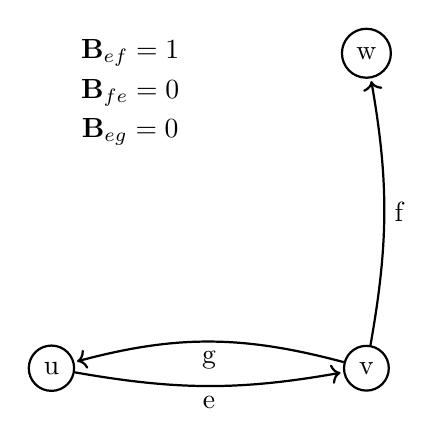
\begin{tikzpicture}[shorten > = 1pt, thick]
		\begin{scope}[every node/.style={circle,thick,draw} ]
			\node (u) at(0,0) {u};
			\node (v) at(4,0) {v};
			\node (w) at(4,4) {w};
		\end{scope}
		\begin{scope}[->],
				every edge/.style={draw=very thick}
			\path[->] (u) edge [bend right = 10] node [below] {e} (v);
			\path[->] (v) edge [bend right = 10] node [right] {f} (w);
			\path[->] (v) edge [bend right = 15] node [below] {g} (u);
		\end{scope}
		\begin{scope}[every node/.style={}]
			\node (bef) at(1, 4) {$\mathbf{B}_{ef}=1$};
			\node (bfe) at(1, 3.5) {$\mathbf{B}_{fe}=0$};
			\node (beg) at(1, 3.0) {$\mathbf{B}_{eg}=0$};
		\end{scope}
	\end{tikzpicture}
	\caption{Havainnekuva NBO:sta. Matriisi $\mathbf{B}$ ei yleisesti ole symmetrinen, kuten $\mathbf{B}_{fe}$ ja $\mathbf{B}_{fe}$ perusteella nähdään.}
	\label{fig:nbo}
\end{figure}

\subsection{Tuloksia}
Yhteisöntunnistusta tutkittin työssä myös simulaatioiden avulla. Simulaatioita varten generoitiin stokastista lohkomallia noudattavia verkkoja, joista pyrittiin laskennallisesti tunnistamaan yhteisöt. Tunnistamisessa käytettiin sekä naapurusmatriisimenetelmää että taaksekääntymättömäään operaattoriin perustuvaa menetelmää. Yhteisöntunnistuksen onnistumista mitattiin laskemalla estimoitujen ja todellisten yhteisöjen välinen korrelaation itseisarvo, eli käytettiin kappaleessa 3 esiteltyä positiiviseen korrelaatioon perustuvaa mittaria.

Ensimmäisenä tutkittiin lohkomallin tiheää tapausta. Tiheässä tapauksessa sekä naapuruusmatriisimenetelmä että taaksekääntymättömään operaattoriin perustuva menetelmä tunnistavat yhteisöt hyvin, kun verkon koko kasvaa. Molemmilla estimoidun ja todellisen yhteisöjaon välisen korrelaation itseisarvo lähestyy yhtä verkon koon kasvaessa, kuten kuvan \ref{fig:dense} perusteella nähdään. Mitä pienempi ero parametreillä $p$ ja $q$ on, sitä suuremman verkon menetelmät kuitenkin tarvitsevat hyvään tunnistustulokseen.

Taaksekääntymätön operaattori on erityisesti tiheässä tapauksessa laskennallisesti huomattavasti naapuruusmatriisimenetelmää raskaampi. Kun verkossa on $n$ solmua, naapuruusmatriisin koko on luonnollisesti $n \times n$, kun taas matriisn $\mathbf{B}$ koko on $O(n^2 \times n^2)$. Tämä merkitsee sitä, että kovin suurilla tiheillä verkoilla sitä ei ole käytännöllistä käyttää. Täten pienempiä parametrien $p$ ja $q$ eroja tutkittiinkin pelkällä naapuruusmatriisimenetelmällä ja suuremmalla verkon koolla. Pienilläkin parametrien eroilla päästään hyviin tunnistustuloksiin, kunhan verkon koon annetaan kasvaa, kuten kuvasta \ref{fig:o_adj_all} nähdään.

\begin{figure}
	\centering
	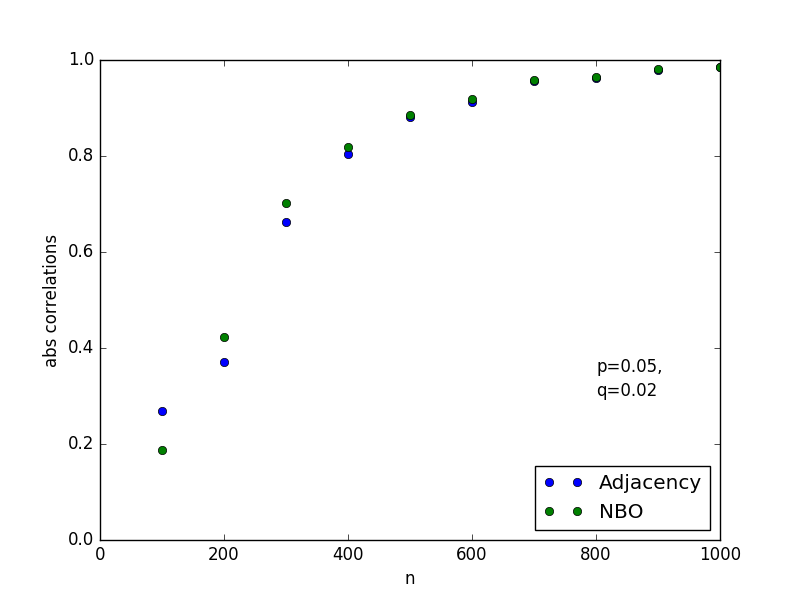
\includegraphics[width = \textwidth]{adj_nbo_den_2.png}
	\caption{Kuvassa tiheän lohkomallin yhteisöntunnistuskorrelaatioita kummallakin menetelmällä. Molemmat menetelmät tunnistavat verkon yhteisöt liki korrelaatiolla 1, kun verkon koko kasvaa.}
	\label{fig:dense}
\end{figure}

\begin{figure}
	\begin{subfigure}{0.3\textwidth}
		\centering
		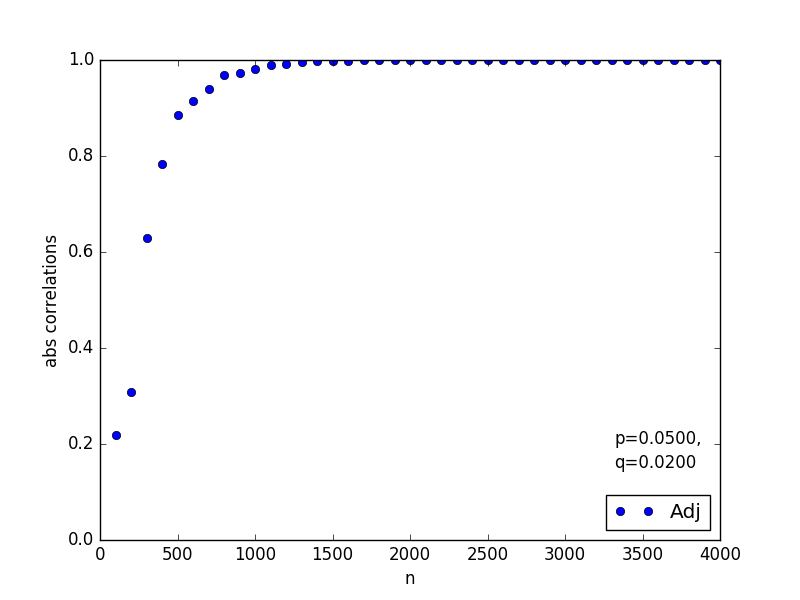
\includegraphics[width=\textwidth]{o_pres_1.png}
		\caption{p = 0.05, q = 0.02}
		\label{fig:o_adj_1}
	\end{subfigure}
	\begin{subfigure}{0.3\textwidth}
		\centering
		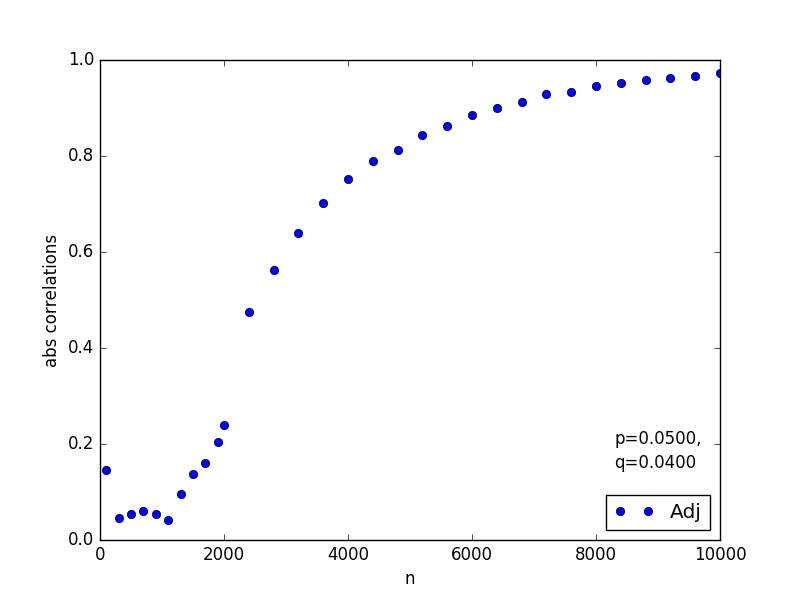
\includegraphics[width=\textwidth]{o_pres_2.png}
		\caption{p = 0.05, q = 0.40}
	\end{subfigure}
	\begin{subfigure}{0.3\textwidth}
		\centering
		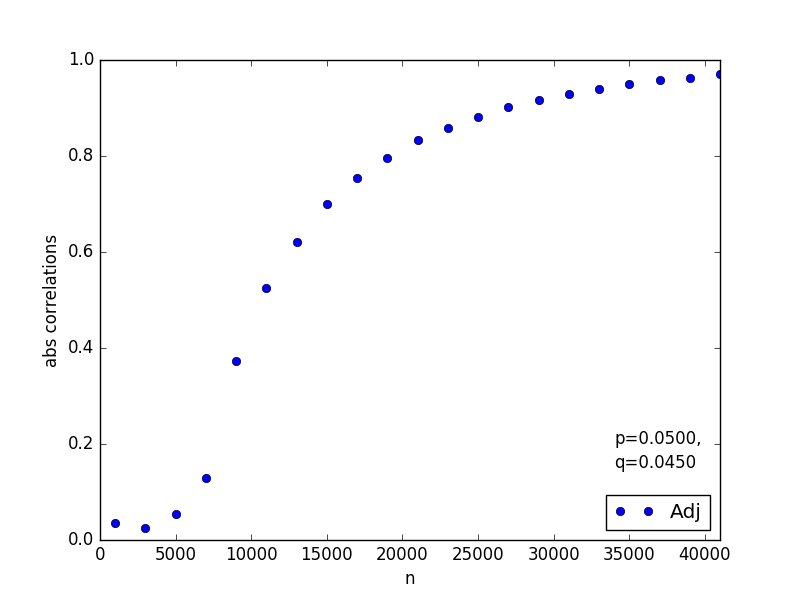
\includegraphics[width=\textwidth]{o_pres_3.png}
		\caption{p = 0.05, q = 0.45}
	\end{subfigure}
	\caption{Kuvissa on eri parametreillä $p$ ja $q$ tutkittu yhteisöntunnistusta lohkomallin tiheässä tapauksessa. Pienempi parametrien erostus vaatii suuremman verkon, jotta yhteisöt pystytään tunnistamaan suurella korrelaatiolla.}
	\label{fig:o_adj_all}
\end{figure}
Harvassa tapauksessa tulokset ovat monipuolisempia. Ensinnäkin huomataan, että selvästi teorian mukaan tunnistettavan puolellakaan olevilla parametrien $a$ ja $b$ arvoilla ei päästä yhtä hyvään tuloseen kummallakaan menetelmällä kuin tiheässä tapauksessa. Tämä on toki luonnollista, sillä tiheän tapauksen pienikin ero parametreissa $p$ ja $q$ vastaa harvaa tapausta tunnistamisen kannalta suotuisilla paramatreillä $a$ ja $b$, kun verkon koko kasvaa tarpeen suureksi. Tuloksia suotuisilla parametreillä on esitelty kuvassa \ref{fig:adj_nbo_sp_easy}. Kuvassa on esimerkki simulaatiotuloksesta, jossa kumpikin tunnistusmenetelmä toimii hyvin.

Teoreemojen \ref{teoreema:mahdottomuus} ja \ref{teoreema:tarkentuvatest} mukainen tunnistusraja tulee esille myös simulaatioissa. Kuvassa \ref{fig:rajatapaus} on esitetty kahden eri simulaation tuloksia. Toisessa osamäärä $\frac{(a-b)^2}{2(a+b)}$ on hieman alle arvon yksi ja toisessa juuri arvon yksi yläpuolella. Osamäärän arvo yksi vastaa yllämainittujen teoreemojen mukaista rajaa. Koska teoreemojen tulos on asymptoottinen, onkin luonnollista että ilmiö tulee paremmin esiin vasta suurella verkon koolla.

Sama raja saadaan esille myös verkon koon pysyessä vakiona ja parametrejä muuttamalla. Kuvassa \ref{fig:a_param} on pidetty verkon koko ja toinen parametreistä $a$ ja $b$ vakioina ja muutettu toista parametreistä. Tällöin huomataan sama rajailmiö, kun parametrien ero muuttuu suotuisammaksi.

Tunnistusmenetelmistä NBO on selvästi tunnistuskyvyltään parempi menetelmä, sillä sen teho säilyy myös verkon koon kasvaessa ja parametrien arvojen muuttuessa lähemmäs tunnistusrajan mahdottomuusaluetta. Harvassa tapauksessa sen tunnistustehon paremmuus tulee selvemmin esillle. Kuitenkin tiheässä tapausessa se on laskennallisesti selvästi raskaampi.

\begin{figure}
	\centering
	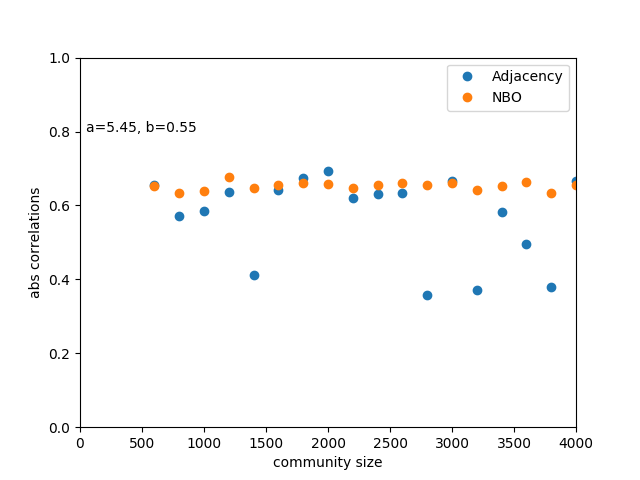
\includegraphics[width = 0.8\textwidth]{adj_nbo_sp_easy.png}
	\caption{Nbo:n ja adj:n vertailua helpoilla a ja b, eli siten että kummallakin menetelmällä päästään kohtuullisen hyvään tulokseen. Ehkä pitäisi olla useampikin kuva hieman eri parametreillä.}
	\label{fig:adj_nbo_sp_easy}
\end{figure}

\begin{figure}
	\label{fig:adj_nbo_sp_hard}
	\centering
		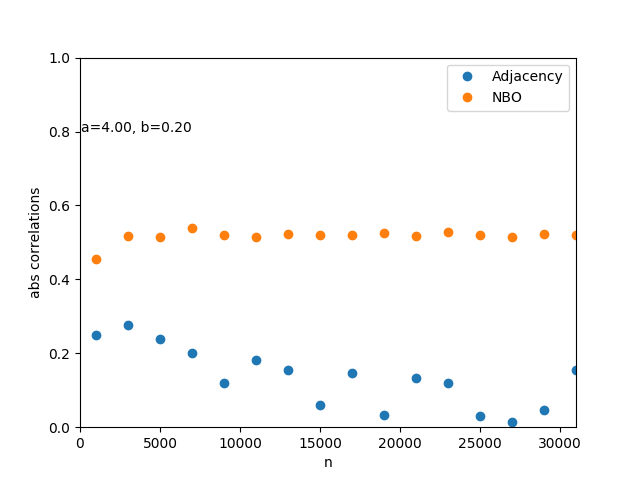
\includegraphics[width = 0.8\textwidth]{adj_nbo_hard_presentation.png}
		\caption{Taaksekääntymättömään operaattoriin perustuva estimaattori tunnistaa yhteisöt noin 0.5 suuruisella korrelaatiolla parametreillä $a = 4.00$ ja $b = 0.20$ verkon koosta riippumatta. Naapuruusmatriisiin perustuvan menetelmän tunnistuskyky heikkenee olemattomiin verkon kasvaessa.}
\end{figure}

\begin{figure}
	\centering
	\begin{subfigure}[b]{0.45 \textwidth}
		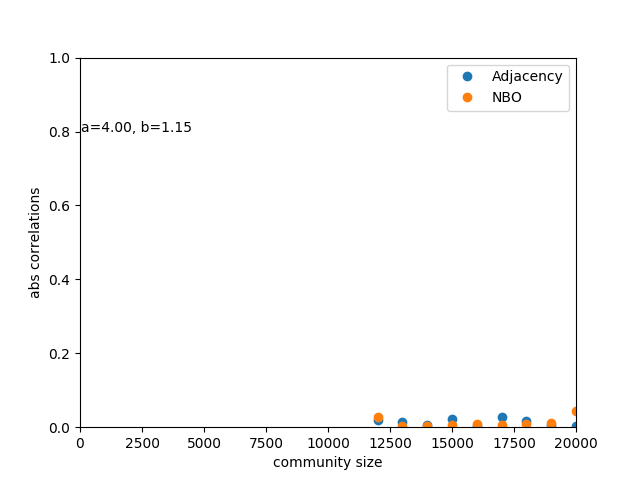
\includegraphics[width = \textwidth]{impossible.png}
		\caption{Juuri mahdottomuusrajan alapuolella. Pos. kor. tunnistus ei onnistu.}
	\end{subfigure}
	\begin{subfigure}[b]{0.45 \textwidth}
		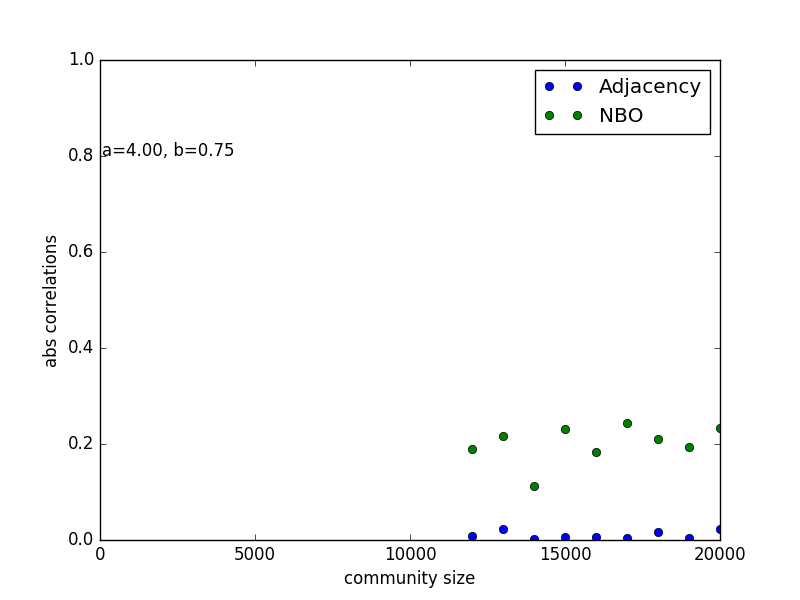
\includegraphics[width = \textwidth]{possible.png}
		\caption{Juuri mahdottomuusrajan yläpuolella. Tunnistaminen onnistuu luotettavasti positiivisella korrelaatiolla NBO:lla, ei kuitenkaan läheskään täydellisesti.}
	\end{subfigure}
	\caption{Nbo:n ja adj:n vertailua mahdottomuusrajan ympäristössä. Rajan alapuolella korrelaatio on 0, yläpuolella se on positiivinen NBO:lla. Paremmat kuvat tulossa.}
	\label{fig:rajatapaus}
\end{figure}

\begin{figure}
	\centering
	\begin{subfigure}[b]{0.45 \textwidth}
		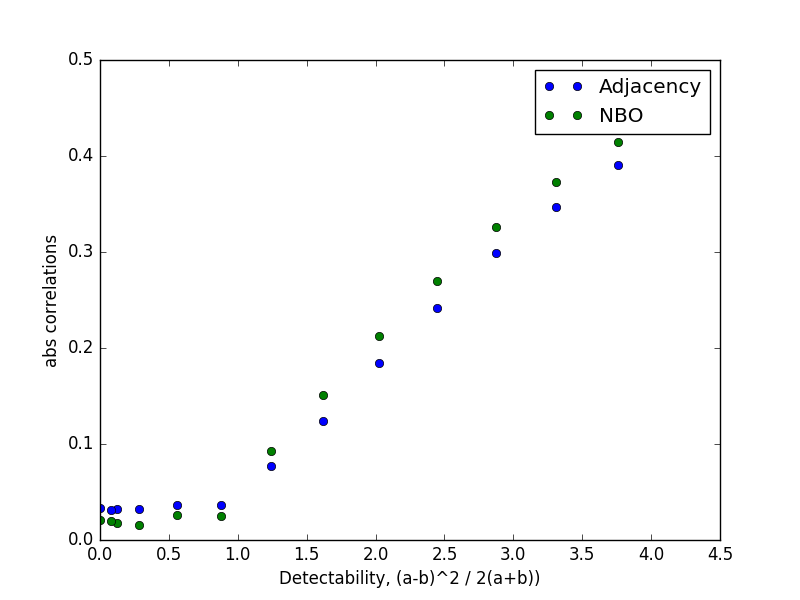
\includegraphics[width = \textwidth]{detectability_a_1.png}
	\end{subfigure}
	\begin{subfigure}[b]{0.45 \textwidth}
		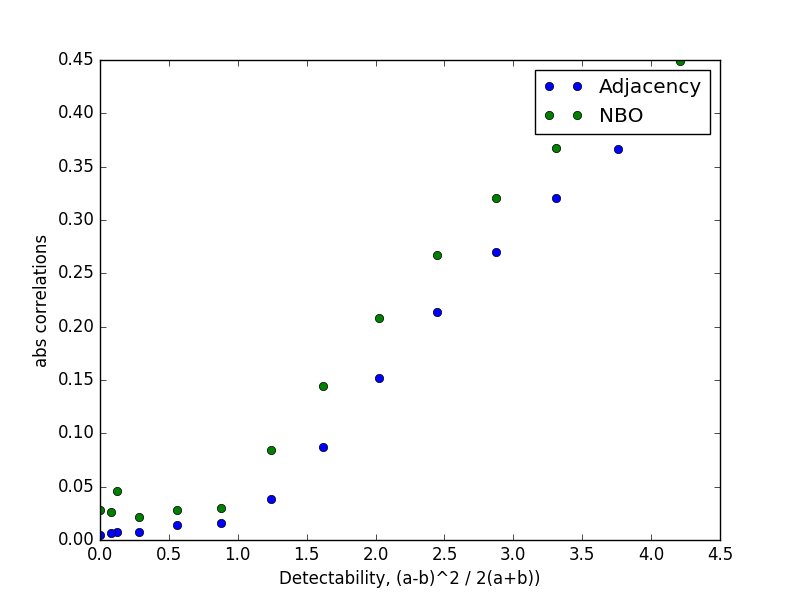
\includegraphics[width = \textwidth]{detectability_a_2.png}
	\end{subfigure}
	\caption{Parametrin $a$ muutos vakio $b$:lla ja kiinteällä $n$:llä. Tunnistaminen alkaa onnistua kun suhde $\frac{(a-b)^2}{2(a+b)}$ saavuttaa arvon 1 ja tunnistaminen onnistuu sitä suuremmilla arvoilla.}
	\label{fig:a_param}
\end{figure}

%\begin{figure}
%	\centering
%	\begin{subfigure}[b]{0.45 \textwidth}
%		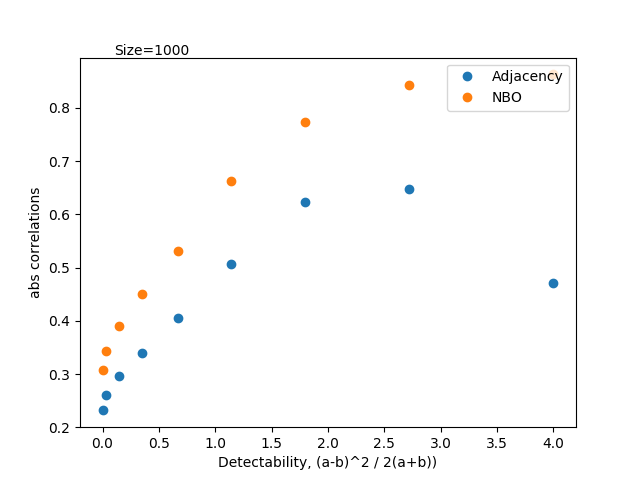
\includegraphics[width = \textwidth]{detectability_b_1.png}
%	\end{subfigure}
%	\begin{subfigure}[b]{0.45 \textwidth}
%		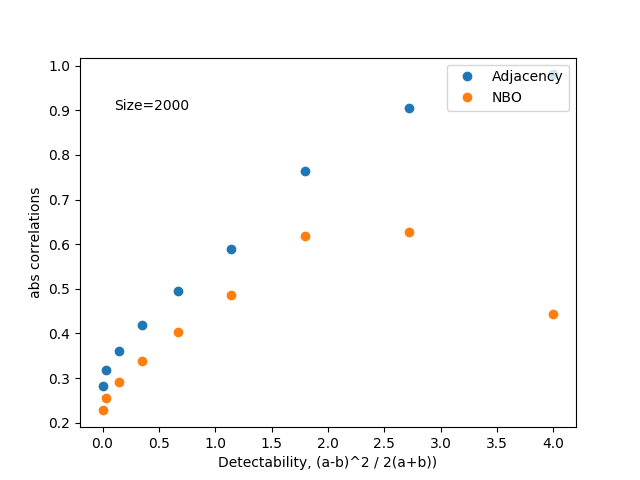
\includegraphics[width = \textwidth]{detectability_b_2.png}
%	\end{subfigure}
%	\caption{Parametrin b muutos vakio a:lla, muuten sama kuin ylempi. Ideana näyttää, että a:n ja b:n välinen suhde on oleellinen, ei pelkästään niiden absoluuttiset arvot. Jostain syystä tuloket eivät vielä täsmää.}
%	\label{fig:b_param}
%\end{figure}

\clearpage
%% Lähdeluettelo

\thesisbibliography

\begin{thebibliography}{99}

%% Alla pilkun jälkeen on pakotettu oikea väli \<välilyönti>-merkeillä.

\bibitem{Hoeffding} Hoeffding,\ W. Probability inequalities for sums of bounded random variables. \textit{Journal of the American Statistical Association} 1963, vol.\ 58, s.\ 13-30.
\bibitem{Fortunato} Fortunato,\ S. Community detection in graphs. \textit{Physics Reports.} 2010, vol.\ 486, s.\ 75-174.
\bibitem{reconstruction} Mossel,\ E., Neeman,\ J., Sly,\ A. Reconstruction and estimation in the planted partition model. \textit{Probability Theory and Related Fields} 2015, vol.\ 162, s.\ 431-461.

\end{thebibliography}

%% Liitteet
\clearpage

\thesisappendix
\end{document}
